\documentclass{article}
\usepackage{amssymb}
\usepackage{amsmath}
\usepackage[T1]{fontenc}
\usepackage[utf8]{inputenc}
\usepackage[unicode=true]{hyperref}
\usepackage{natbib}
\bibliographystyle{plainnat}
\usepackage{listings}
\usepackage{booktabs}
\usepackage{graphicx}


\begin{document}

\section{Sections \& Paragraphs}

Lorem ipsum dolor sit amet, consectetur adipiscing elit. Curabitur
pharetra enim ut eros pharetra, in varius nunc commodo. Curabitur sed
tellus efficitur, pretium sapien et, auctor urna. Class aptent taciti
sociosqu ad litora torquent per conubia nostra, per inceptos himenaeos.
Mauris id maximus sapien. Praesent malesuada sem sed felis volutpat
porttitor. Aenean commodo cursus metus, in laoreet lacus tincidunt vel.
Praesent a quam eu mauris lacinia viverra. Proin aliquet, risus nec
interdum laoreet, leo dolor dapibus neque, ac fermentum libero urna
posuere mauris. Ut quis ullamcorper ante, ut vulputate erat. Nulla
condimentum sagittis dui, vitae facilisis mi blandit nec. Cras id
suscipit enim.

\subsection{Subsection}

Cras enim nisi, molestie quis neque vel, aliquet laoreet metus. Maecenas
ut venenatis leo. Suspendisse malesuada ligula maximus, varius lorem
sed, ullamcorper tellus. Vestibulum turpis nisi, pellentesque in dictum
at, finibus sit amet ligula. Mauris fermentum pharetra dolor lacinia
vestibulum. Nunc eget feugiat mauris, ac posuere erat. Pellentesque a
rhoncus justo, at consectetur elit. Sed condimentum, ligula sit amet
hendrerit viverra, dolor mi dictum turpis, sit amet accumsan arcu urna
et sapien. Donec rutrum hendrerit mauris, eu faucibus purus rhoncus
vitae. Aliquam vitae pellentesque dolor, non tempus nulla. Etiam vitae
justo tortor. Aenean sodales eu lorem eu luctus.

\subsubsection{Subsubsection}

In euismod neque ut purus pellentesque tincidunt. Nullam bibendum
sagittis ultrices. Nunc nunc arcu, maximus nec lorem et, auctor lacinia
ante. Donec dapibus scelerisque ante, at pulvinar odio euismod non. Nam
in consequat diam, quis auctor diam. Praesent at luctus felis. Vivamus
gravida finibus iaculis. Nunc turpis erat, ullamcorper eu fringilla ac,
faucibus eu eros.

\subsection{Formating}

You can write text with different \emph{emphasis}. For really important
stuff, you can even have \textbf{strong emphasis}.

Subscript as in H\textsubscript{2}O is possible. So is superscript:
2\textsuperscript{10}.

\section{Math}

You can write math as part of a sentence. For example, did you know that
$1+2=3$?

You can also have math in blocks:

$$e = mc^2$$

Also like this:

\begin{equation}
e = mc^2
\end{equation}

\section{References}

Blah blah \citetext{\citealp[see][pp.~33-35]{doe99}; \citealp[also][chap. 1]{smith04}}.

Blah blah \citep[pp.~33-35 and 38-39]{doe99}.

Blah blah \citep{smith04, doe99}.

Smith says blah \citeyearpar{smith04}.

\citet{smith04} says blah.

\citet[p.~33]{smith04} says blah.

\section{Code}

\subsubsection{Inline code}

Lorem ipsum dolor sit amet, consectetur adipiscing elit.
\lstinline!x <- stats::rnorm(n)! Curabitur pharetra enim ut eros
pharetra, in varius nunc commodo. Curabitur sed tellus efficitur,
pretium sapien et, auctor urna.

\subsubsection{Code without highlighting}

\begin{lstlisting}
for(i in 1:5) print(1:i)
for(n in c(2,5,10,20,50)) {
   x <- stats::rnorm(n)
   cat(n, ": ", sum(x^2), "\n", sep = "")
}
f <- factor(sample(letters[1:5], 10, replace = TRUE))
for(i in unique(f)) print(i)
\end{lstlisting}

\subsubsection{Code with highlighting}

\begin{lstlisting}[language=R]
for(i in 1:5) print(1:i)
for(n in c(2,5,10,20,50)) {
   x <- stats::rnorm(n)
   cat(n, ": ", sum(x^2), "\n", sep = "")
}
f <- factor(sample(letters[1:5], 10, replace = TRUE))
for(i in unique(f)) print(i)
\end{lstlisting}

\section{Figures}

\begin{figure}
\centering
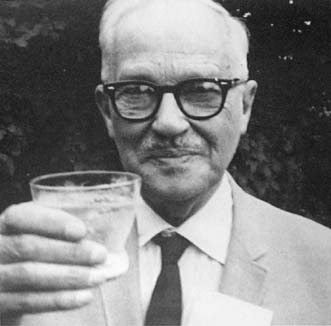
\includegraphics{example-latex/neyman.jpg}
\caption{This is Neyman}
\end{figure}

\section{Footnotes}

Cras enim nisi, molestie quis neque vel, aliquet laoreet
metus.\footnote{Maecenas ut venenatis leo. Suspendisse malesuada ligula
  maximus, varius lorem sed, ullamcorper tellus.} Vestibulum turpis
nisi, pellentesque in dictum at, finibus sit amet ligula. Mauris
fermentum pharetra dolor lacinia vestibulum.\footnote{Nunc eget feugiat
  mauris, ac posuere erat.} Pellentesque a rhoncus justo, at consectetur
elit. Sed condimentum, ligula sit amet hendrerit viverra, dolor mi
dictum turpis, sit amet accumsan arcu urna et sapien. Donec rutrum
hendrerit mauris, eu faucibus purus rhoncus vitae. Aliquam vitae
pellentesque dolor, non tempus nulla. Etiam vitae justo tortor. Aenean
sodales eu lorem eu luctus.

\section{Links}

If you want the link and the text to be the same, just write:
\url{http://google.com}.

If you want the link text to be different from the link, write:
\href{http://google.com}{Google}.

\section{Block quotations}

Lorem ipsum dolor sit amet, consectetur adipiscing elit. Curabitur
pharetra enim ut eros pharetra, in varius nunc commodo. Curabitur sed
tellus efficitur, pretium sapien et, auctor urna. Class aptent taciti
sociosqu ad litora torquent per conubia nostra, per inceptos himenaeos.

\begin{quote}
Mauris id maximus sapien. Praesent malesuada sem sed felis volutpat
porttitor. Aenean commodo cursus metus, in laoreet lacus tincidunt vel.
\end{quote}

Praesent a quam eu mauris lacinia viverra. Proin aliquet, risus nec
interdum laoreet, leo dolor dapibus neque, ac fermentum libero urna
posuere mauris. Ut quis ullamcorper ante, ut vulputate erat. Nulla
condimentum sagittis dui, vitae facilisis mi blandit nec. Cras id
suscipit enim.

\section{Lists}

\subsubsection{Bullet lists}

\begin{itemize}
\item Bullet 1
\item Bullet 2
\item Bullet 3
\item Bullet 4
\end{itemize}

\subsubsection{Ordered lists}

\begin{enumerate}
\item Ordered 1
\item Ordered 2
\item Ordered 3
\item Ordered 4
\end{enumerate}

\section{Tables}

\begin{table}
	\centering
	\caption{An example of a table.}
	\begin{tabular}{ r l l c }
		Right & Left & Default & Center \\
		12 & 12 & 12 & 12 \\
		123 & 123 & 123 & 123 \\
		1 & 1 & 1 & 1 \\
	\end{tabular}
\end{table}

\end{document}
